\subsection{Terrain-Transformationen}
Nachdem das Layout der Welt mittels Space-Partitioning~\ref{WG:SpacePartitioning} berechnet wurde und dieses anschließend in entsprechende Terrain Masken\todo{add ref to section} unterteilt wurde, muss die Welt nun in Unity generiert werden.
Die Basis dafür bildet das Unity Terrain Objekt.
Um das Terrain aus dem Welt-Layout prozedural zu generieren, werden sukzessive die verschiedenen Operationen\todo{add ref} auf den Teilen der Heightmap ausgeführt, die durch die Terrain-Masken vorgegeben werden.
Die folgenden Transformationen werden in dieser Reihenfolge auf Teilen der Heightmap ausgeführt:
\begin{enumerate}
    \item \texttt{SetByMask}: Die Räume und Korridore des Space-Partitioning werden in der Heightmap umgesetzt. Dies geschieht einmalig am Anfang und bildet die Grundlage für das Welt-Layout. %, indem an den Koordinaten wo ein Raum oder ein Korridor platziert wurde
    \item \texttt{AverageFilter}: Ausgehend von Schritt 1 ist die Trennung vom begehbaren Bereich (Räume und Korridore) und den Bergen im Terrain eine scharfe Kante.
          Die Heightmap springt an den Begrenzungen von 0 auf 1, was im Spiel unnatürlich aussieht.
          Um diese Übergänge zu glätten wird der \texttt{AverageFilter} 600-mal auf den nicht-begehbaren Bereich angewandt.
          Dies sorgt dafür, dass eine glatte Kante zwischen den Räumen und Korridoren und den Bergen entsteht.
    \item \texttt{PerlinNoise}: Damit die Berge eine natürliche Struktur erhalten, wird auf diesen Bereichen 3-mal ein Perlin Noise angewandt.
          Diese Anwendung des Perlin Noise lässt die hohen Berge entstehen.
    \item \texttt{Power}: Um die Höhenunterschiede in den Bergen zu verstärken, wird an jedem Punkt der Wert der Heightmap einmal mit $3$ potenziert.
    \item \texttt{PerlinNoise}: Ausgehend davon, wird nochmals auf den Bergen 2-mal ein Perlin Noise angewandt, welches Berge entstehen lässt, die etwas kleiner sind.
    \item \texttt{AverageFilter}: Um die Korridore und Räume herum, wird ein 6 Einheiten breiter Bereich geglättet.
          Um dies zu erreichen, wird der \texttt{AverageFilter} 15-mal dort angewandt.
    \item \texttt{SetByMask}: Zum Schluss wird um die Korridore und Räume ein 1 Einheiten breiter Bereich leicht erhöht, um die Berge besser zu trennen.
\end{enumerate}

Eine Herausforderung bei der Umsetzung dieser Idee ist, dass diese Operationen auf allen, von der jeweiligen Maske vorgegebenen, Punkten ausgeführt werden müssen.
Besonders bei größeren Heightmaps ist dies problematisch, da beispielsweise für eine Heightmap mit einer Seitenlänge von 1024, Operationen auf bis zu 1.048.576 Punkten ausgeführt werden müssen.
Rechenintensive Operationen, wie der \texttt{AverageFilter} werden zwar nur auf einer Teilmenge der Punkte ausgeführt, jedoch besteht dabei auch das Problem, dass der Filter sehr oft angewandt werden muss.
Damit die Welt auch zur Laufzeit generiert werden kann, ohne dass dies zu sehr langen Ladezeiten führt, ist es wichtig, dass die einzelnen Operationen effizient implementiert werden.


\subsubsection{Implementation der Terrain-Transformationen}
Eine zentrale Beobachtung bei der Implementation der Transformationen ist, dass die Operationen auf den einzelnen Punkten der Heightmap, alle unabhängig voneinander ausgeführt werden können.
Die einzige Abhängigkeit besteht zwischen den einzelnen Anwendungen einer Operation.
Dies führt dazu, dass sich die Operationen effizient parallelisieren lassen.
Insgesamt wurden fünf Versionen der Terrain-Transformationen implementiert:

Um die Ideen der verschiedenen Transformations-Operationen auszuprobieren, wurden zunächst Funktionen implementiert, die nahezu beliebige Operationen auf Punkten der Heightmap ausführen, die von einer Maske vorgegeben werden.
Diese Funktionen iterieren über alle Punkte der Heightmap und prüfen dabei, ob der aktuelle Punkt in der Maske liegt.
Ist dies der Fall, wird die Operation auf dem Punkt ausgeführt.
Eine Besonderheit ist, dass in dieser Version die Implementation des \texttt{AverageFilter}, nicht auf den 3x3 \texttt{AverageFilter} beschränkt ist, sondern dass die Funktion, Filter beliebiger Größe und Form auf die Heightmap anwenden kann.
Diese Implementation wurde genutzt um herauszufinden, welche Transformationen sinnvoll sind.
Die Ausführung dieser Version der Operationen erfolgt stets sequenziell und ausschließlich auf der CPU.

Nachdem die gewünschten Transformationen identifiziert und implementiert wurden, musste der \texttt{AverageFilter} effizient implementiert werden, da dieser die meiste Rechenzeit in Anspruch nimmt.
Da diese Operation sehr häufig (bis zu 600-mal) wiederholt wird und vollständig parallelisiert werden kann, ist es naheliegend für den \texttt{AverageFilter} einen ComputeShader für die Ausführung auf einer Grafikkarte zu schreiben.
Ein ComputeShader ist eine Funktion, die beispielsweise auf einer Grafikkarte ausgeführt werden kann.
Hierbei wird pro Funktionsaufruf jeweils ein Datenpunkt übergeben und auf einer Recheneinheit der Grafikkarte ausgeführt.
Es werden stets Gruppen von Datenpunkten übergeben, die gleichzeitig ausgeführt werden.
Zusätzlich zur Implementation des \texttt{AverageFilter} in einem ComputeShader, müssen die Daten, auf die die Grafikkarte zugreifen soll, erst noch so vorbereitet werden, dass diese in den Speicher der Grafikkarte geladen werden können.
\begin{listing}
    \begin{minted}[linenos,tabsize=2,breaklines,fontsize=\small]{hlsl}
        static const float avg_3x3 = 1/(float)9;
        [numthreads(256,1,1)]
        void AverageFilterAdd3x3 (uint3 id : SV_DispatchThreadID) {
            uint item = _work_items[id.x];
            if (id.x >= _work_item_count) return;
            uint row = item / _size_input;
            uint col = item % _size_input;
            float sum = 0;
            sum += _input[(row - 1) * _size_input + (col - 1)] * avg_3x3;
            sum += _input[(row - 1) * _size_input + (col)] * avg_3x3;
            sum += _input[(row - 1) * _size_input + (col + 1)] * avg_3x3;
            sum += _input[(row)*_size_input + (col - 1)] * avg_3x3;
            sum += _input[(row)*_size_input + (col)] * avg_3x3;
            sum += _input[(row)*_size_input + (col + 1)] * avg_3x3;
            sum += _input[(row + 1) * _size_input + (col - 1)] * avg_3x3;
            sum += _input[(row + 1) * _size_input + (col)] * avg_3x3;
            sum += _input[(row + 1) * _size_input + (col + 1)] * avg_3x3;
            _output[row * _size_input + col] = sum;
        }
    \end{minted}
    \caption{ComputeShader für den \texttt{AverageFilter}.}
    \label{WG:averagefiltershader}
\end{listing}
Listing~\ref{WG:averagefiltershader} zeigt den Programmcode des ComputeShaders für den \texttt{AverageFilter}.
Da häufige Fallunterscheidungen auf einer Grafikkarte ineffizient sein können, wird hier die Terrain-Maske nicht übergeben und für jeden Datenpunkt überprüft, sondern es werden direkt nur die Punkte der Heightmap bearbeitet, die auch in der Maske enthalten sind.
Zudem wird die zweidimensionale Heightmap in ein eindimensionales Array umgewandelt und dementsprechend anders adressiert.
Diese Umwandlungen und das Laden der linearisierten Heightmap auf die Grafikkarte müssen einmalig zum Start der \texttt{AverageFilter} Operation ausgeführt werden.
Da der Filter häufiger nacheinander ausgeführt wird und nicht jedes Mal die Daten konvertiert werden sollen, kann der \texttt{AverageFilter} Funktion direkt die Anzahl an Wiederholungen übergeben werden.
Damit das Ergebnis-Array nicht nach jeder Ausführung von der Grafikkarte zurück in den Hauptspeicher kopiert werden muss, werden im Speicher der Grafikkarte für Platz für ein Eingabe-Array und ein Ausgabe-Array alloziert.
In jeder Iteration werden die Ein- und Ausgabe-Arrays vertauscht, sodass die Daten der Heightmap zwischen den Iterationen nie den Speicher der Grafikkarte verlassen müssen.
Dies würde die Laufzeit erheblich verlängern.

Die dritte Optimierung der Terrain-Transformationen umfasst parallelisierte Versionen der anderen Operationen.
Diese werden jedoch auf der CPU ausgeführt, da der Overhead für die Vorbereitung der Daten für die Grafikkarte zu hoch ist.
Der Programmcode für die einzelnen Operationen verändert sich hier nicht stark, da die \texttt{for}-Schleifen einfach durch \texttt{Parallel.For} Konstrukte ersetzt werden können.
Hierdurch werden die zu verarbeitenden Daten in Gruppen unterteilt und auf der CPU parallel verarbeitet.

Ein Problem, bei der Nutzung eines ComputeShaders ist, dass dieser eine geeignete Grafikkarte voraussetzt.
Im Laufe des Projekts ist es aufgefallen, dass beispielsweise beim Trainieren der Kreaturen auf dem LiDO3, die Grafikkarte nicht zum Generieren der Welt verwendet werden konnte.
Wenn Unity ohne Bildschirm gestartet wurde (headless), trat dieses Problem auch auf.
Aus diesem Grund musste auch eine performante Version des \texttt{AverageFilter} implementiert werden, der nur auf der CPU ausgeführt wird.
Dazu wurde zunächst der Programmcode der ursprünglichen Filter-Operation mittels \texttt{Parallel.For} Konstrukten auf der CPU parallelisiert.
Diese Funktion dient als Ersatz für den ComputeShader, falls keine Grafikkarte verfügbar ist, oder diese den ComputeShader nicht unterstützt.
Die Laufzeit dieser Implementation war zwar für das Training akzeptabel, aber schlechter geeignet, falls im echten Spiel der ComputeShader nicht unterstützt würde.
Die aktuelle Implementation des \texttt{AverageFilter} verwendet den Unity \textit{Burst}-Compiler, um hochoptimierten Programmcode für den Filter zu erzeugen.
Der \textit{Burst}-Compiler verwendet das Unity Job System, indem einzelne Funktionen als Jobs definiert und als Gruppen parallel auf der CPU ausgeführt werden können.
Das Vorgehen ist hier ähnlich wie bei den ComputeShadern.
Der große Vorteil des \textit{Burst}-Compilers ist, dass dieser aus einem Job hochoptimierten code generieren kann, der zudem automatische Vektorisierung auf der CPU unterstützt.
Der Compiler erzeugt automatisch Maschinencode, welcher Vektorinstruktionen der CPU verwendet, um mehrere Datenpunkte gleichzeitig auf einem Kern zu verarbeiten.
Dies erfolgt zusätzlich zur Parallelisierung auf mehreren Kernen der CPU.

\subsubsection{Laufzeitmessungen}
Um die einzelnen Implementationen zu vergleichen und zu evaluieren, ob die Optimierungen auch wirklich zu einer verbesserten Laufzeit führen, wurden Messungen für alle Implementationen durchgeführt.
Die folgenden Messungen wurden alle auf einem PC durchgeführt, der über $\SI{32}{\giga\byte}$ RAM verfügt und einen Intel Core i7-5820k (6 Kerne/12 Threads) sowie eine NVIDIA GTX 780 Ti enthält.
Die Größe der Heightmap der generierten Welt ist 1024x1024, was einer Fläche von ungefähr ${\SI{1}{\kilo\meter}}^2$ entspricht.
Dies ist auch die Größe der Welt im Spiel.
Die Messungen sind in Abbildung~\ref{fig:WG::Shader} dargestellt.

\begin{figure}[ht]
    \centering
    \begin{tikzpicture}
        \begin{axis}[
                % bar shift=-5pt,
                table/search path={chapters/05_Technische_Umsetzung/03_World_Generation/Performance},
                % ybar stacked,
                xbar,
                % bar width=4pt,
                xmin=0,
                nodes near coords,
                % every node near coord/.append style={font=\small},
                nodes near coords style={/pgf/number format/.cd,fixed,fixed zerofill,precision=1},
                % xmax=20,
                axis x line*=bottom,
                axis y line*=none,
                width=.9\linewidth,
                height=6cm,
                xtick distance=30,
                % ytick={0,0.2,...,1},
                minor grid style={dotted,black!60},
                minor tick num=1,
                xmajorgrids=true,
                xminorgrids=true,
                yminorgrids=false,
                xlabel={Laufzeit [s]},
                minor y tick style={draw=none},
                symbolic y coords={5,4,3,2,1},
                ytick={1,2,3,4,5},
                % xticklabels={(1),(2),(3),(4),(5)},
                yticklabels={ST,GPU,\textbf{GPU+MT},CPU+MT,\textbf{Burst+MT}},
                % xticklabel style={xshift=4.5pt,rotate=45,anchor=east,font=\footnotesize},
                % ytick align=center,
                yticklabel style={font=\small},
                % xticklabels={},
                % bar width=7pt,
                % legend style={
                %         at={(0.5,1.1)},
                %         anchor=north,
                %         legend columns=-1,
                %         fill=white,
                %         align=left,
                %         % font=\small,
                %         minimum height=.42cm
                %     }
            ]
            % \addplot[red,semithick,fill=red,fill opacity=0.5,text opacity=1] table [x={filter}, y={test},col sep=comma]{shader2048.csv};
            % \addlegendentry{2048x2048};

            \addplot[blue,semithick,fill=blue,fill opacity=0.5,text opacity=1] table [x={filter}, y={test},col sep=comma]{shader1024.csv};
            % \addlegendentry{1024x1024};

            % \addplot[blue,semithick,fill=blue,fill opacity=0.5,text opacity=1] table [x={filter}, y={test},col sep=comma]{shader512.csv};
            % \addlegendentry{512x512};
        \end{axis}
    \end{tikzpicture}
    \caption[Laufzeit Terrain-Transformationen]{Messungen der Laufzeiten für die Terrain-Transformationen.}\label{fig:WG::Shader}
\end{figure}

Zunächst lässt sich erkennen, dass die initiale, sequenzielle, Implementation (ST) mit einer Laufzeit von über einer Minute sehr viel Zeit beansprucht.
Diese Version ist ungeeignet um die Welt beim Start des Spiels in einem Ladebildschirm zu generieren.
Sobald der \texttt{AverageFilter} auf der Grafikkarte ausgeführt wird (GPU), ist die Laufzeit mit $\SI{1.3}{\second}$ allerdings sehr gut.
Die weitere Parallelisierung der anderen Operatoren (GPU+MT) sorgt für die kürzeste Generierungsdauer von nur $\SI{1}{\second}$.
Die Ausführungszeit für den naiv parallelisierten \texttt{AverageFilter} auf der CPU (CPU+MT), ist mit $\SI{3.9}{\second}$ akzeptabel, aber erheblich langsamer als die Version die ComputeShader verwendet.
Mit einer Laufzeit von $\SI{1.8}{\second}$ ist die Implementation die den \textit{Burst}-Compiler verwendet (Burst+MT) schnell genug, um als Ersatz für die ComputeShader zu dienen, falls diese nicht unterstützt werden.
Die Messungen der Laufzeiten zeigen, dass die Optimierungen der Terrain-Transformationen es erlauben, die Welt stets prozedural beim Start des Spiels zu generieren.

\subsection{L-System Vegetation}
Das in~\ref{sec:L-System} beschriebene L-System wird verwendet um die Welt mit prozedural generierten Pflanzen zu befüllen.
Diese dienen als Hindernisse für den Spieler und die Kreaturen.
Die Pflanzen werden zur Laufzeit aus vordefinierten L-Systemen zur Laufzeit erzeugt und in der Welt platziert.
Für jedes Objekt wird zunächst das L-System ausgewertet, sodass eine Liste von Tupeln mit Start- und Endpunkten der Segmente entsteht.
Ähnlich wie in Abschnitt~\ref{sec:lsystemskel} beschrieben, wird nun für jedes Segment ein primitives Mesh erzeugt, welche zusammen die Pflanze darstellen.
Eine Auswahl an Bäumen die durch L-Systeme erzeugt werden, ist in Abbildung~\ref{fig:Trees} zu sehen.
\begin{figure}[ht]
    \begin{subfigure}[t]{.3\textwidth}
        \centering
        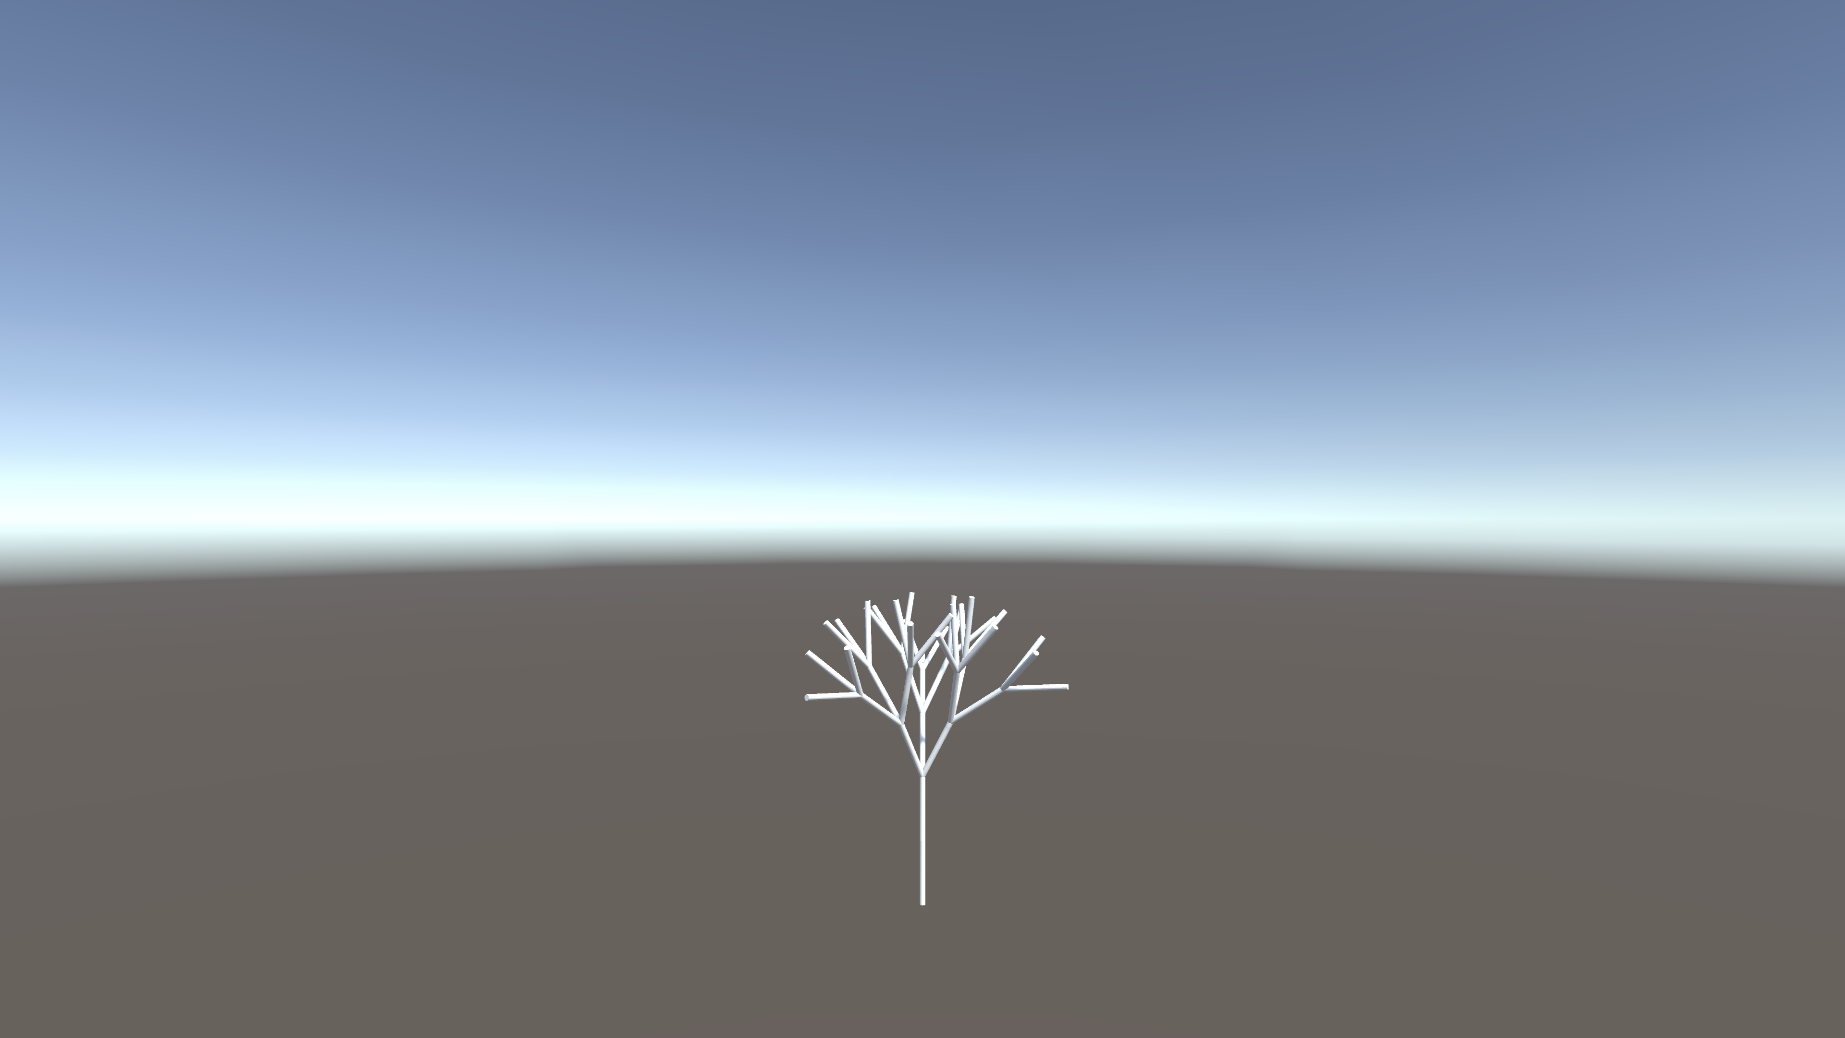
\includegraphics[width=\linewidth]{chapters/05_Technische_Umsetzung/03_World_Generation/Performance/small.png}
        \caption*{Kleiner Baum}
    \end{subfigure}
    \hfill
    \begin{subfigure}[t]{.3\textwidth}
        \centering
        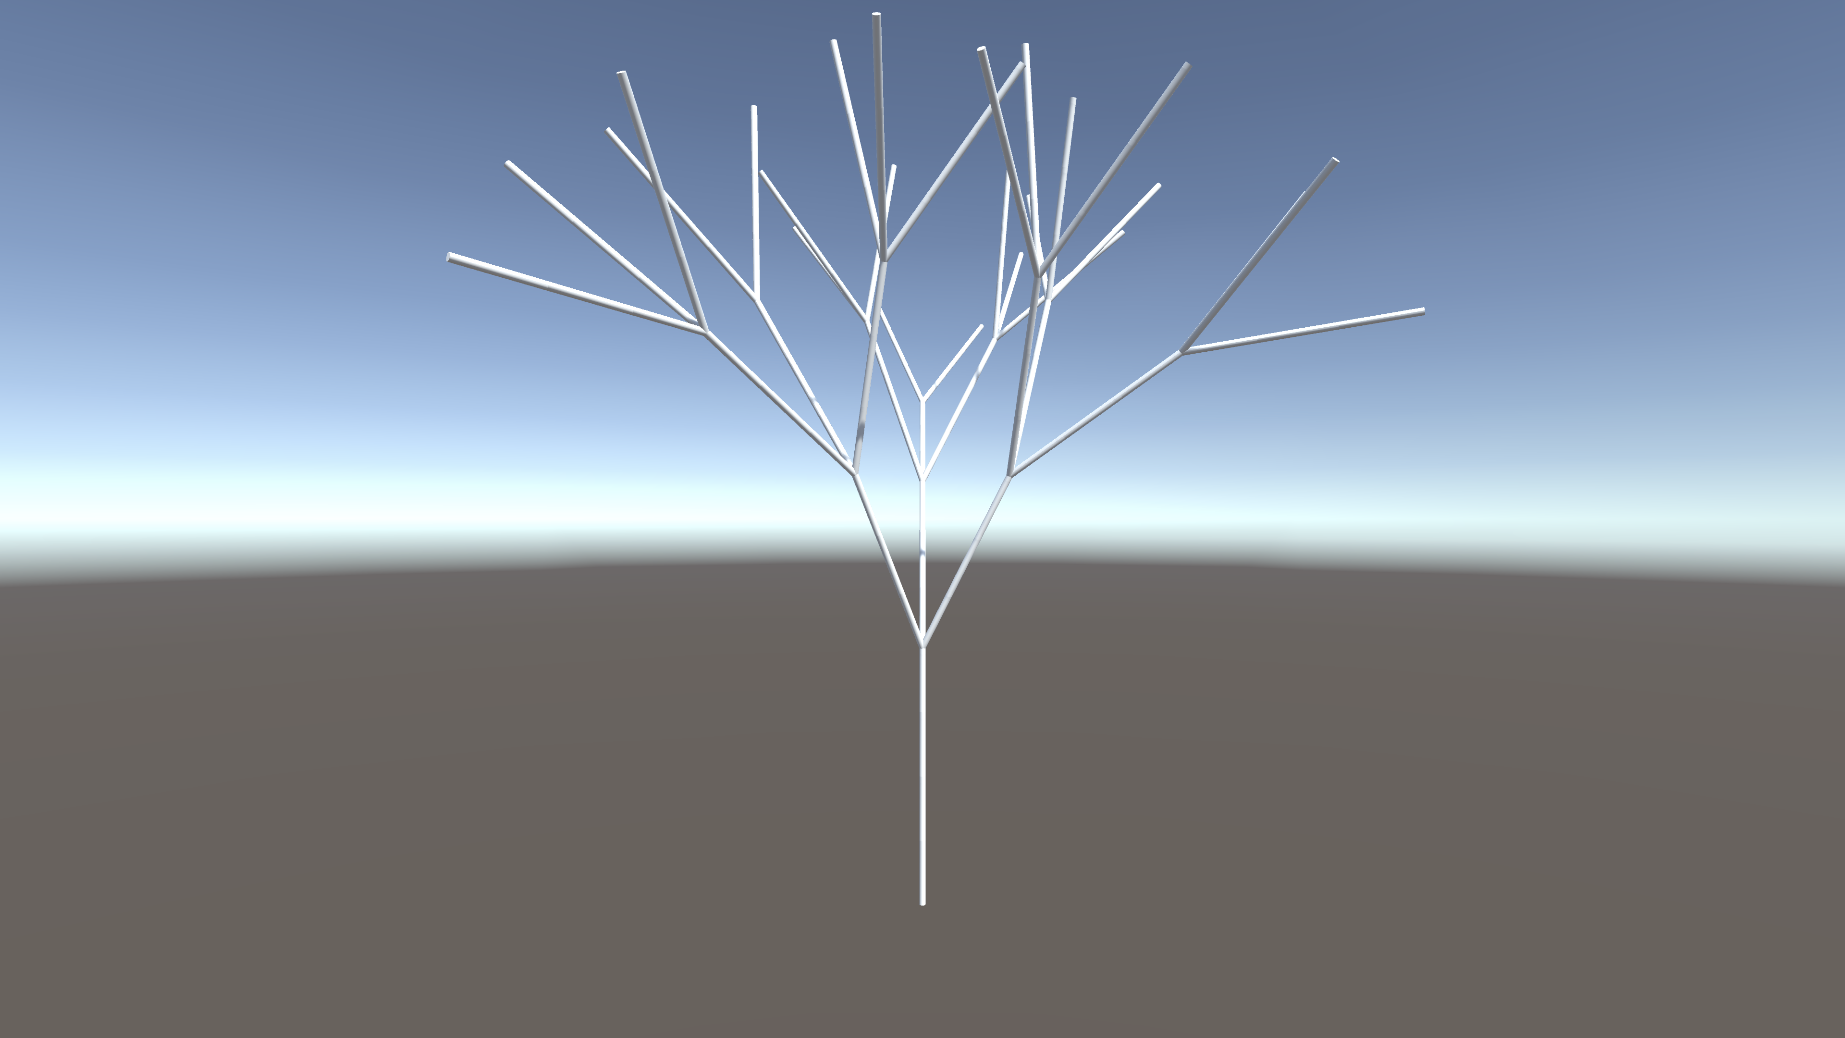
\includegraphics[width=\linewidth]{chapters/05_Technische_Umsetzung/03_World_Generation/Performance/big.png}
        \caption*{Großer Baum}
    \end{subfigure}
    \hfill
    \begin{subfigure}[t]{.3\textwidth}
        \centering
        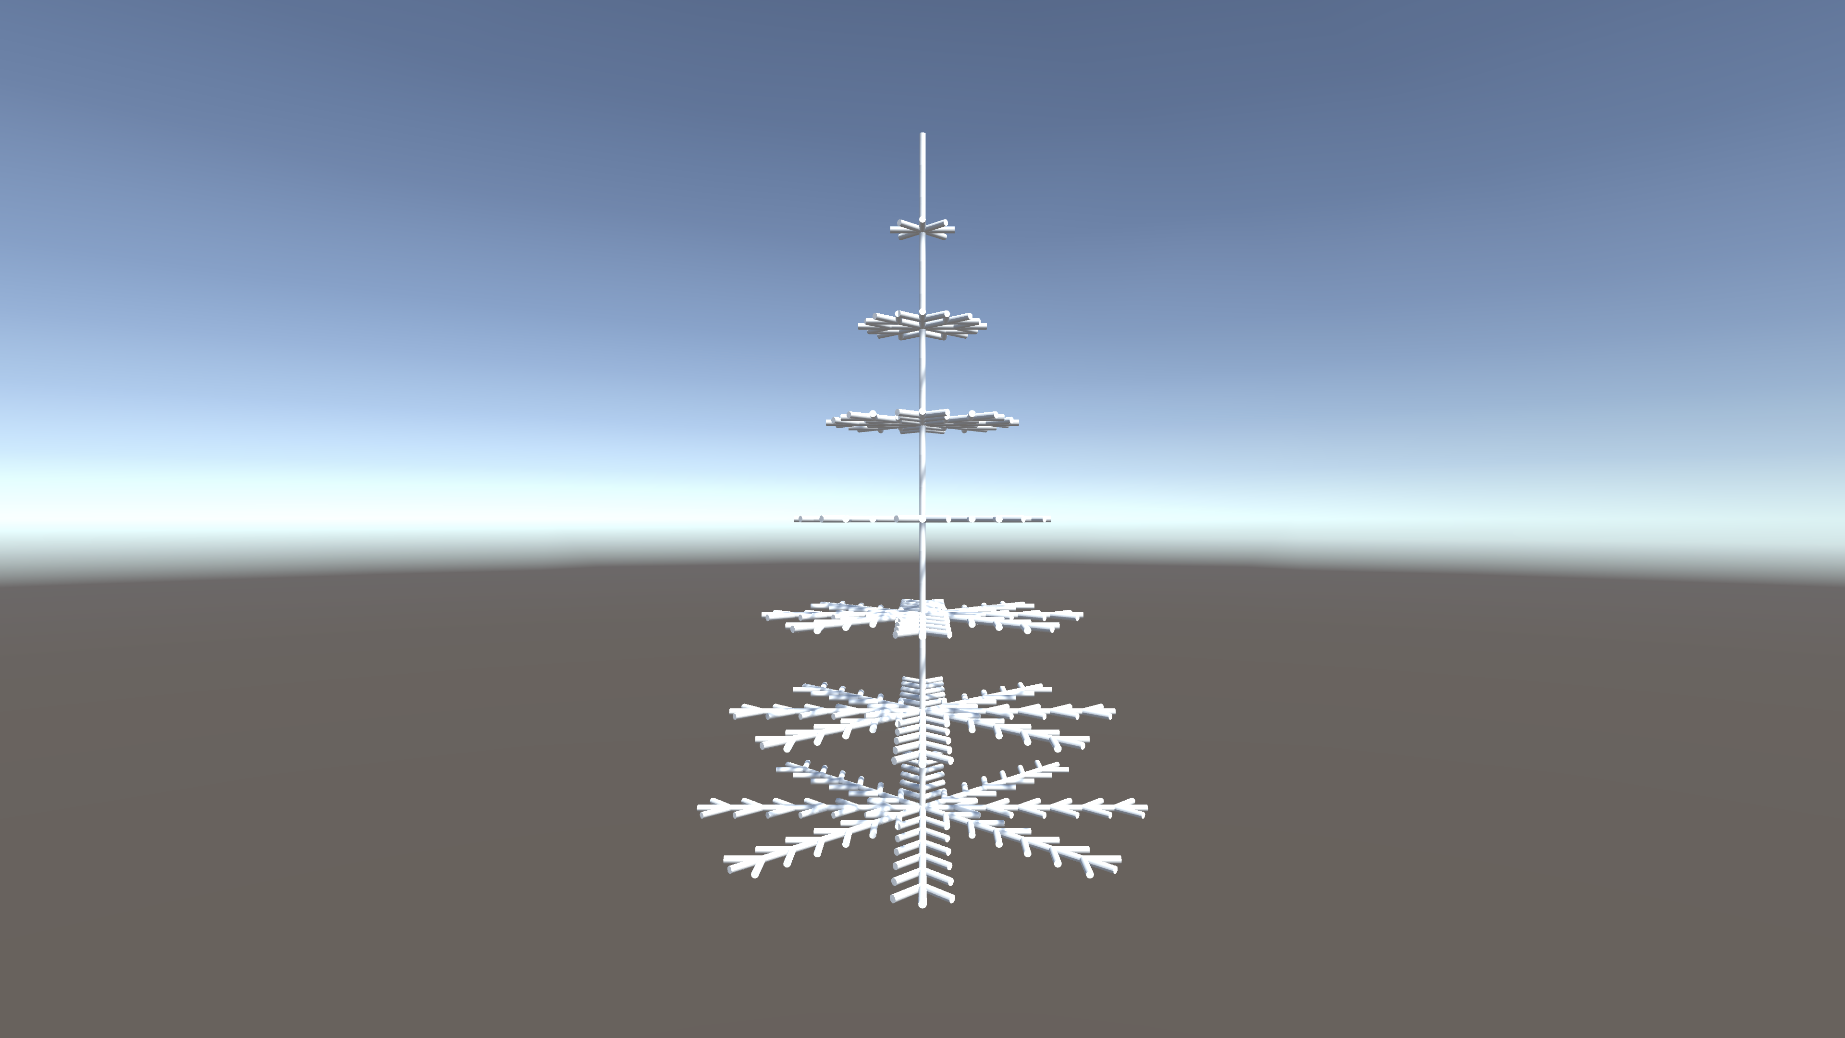
\includegraphics[width=\linewidth]{chapters/05_Technische_Umsetzung/03_World_Generation/Performance/tannenbaum.png}
        \caption*{Tannenbaum}
    \end{subfigure}
    \caption{Bäume die durch L-Systeme erzeugt werden.}\label{fig:Trees}
\end{figure}


\paragraph*{Auswirkungen auf die Leistung}
Die Bäume fügen dem Level einiges an komplexer Geometrie hinzu, sodass darauf geachtet werden muss, dass die Leistung nicht zu stark einbricht und das Spiel spielbar bleibt.
Um dem entgegenzuwirken wurden verschiedene Optimierungen vorgenommen und die Auswirkungen auf die Leistung gemessen.
Als Grundlage für die Messungen dient die in Abbildung~\ref{fig:Vegetationscene} dargestellte Szene.
\begin{figure}[ht]
    \centering
    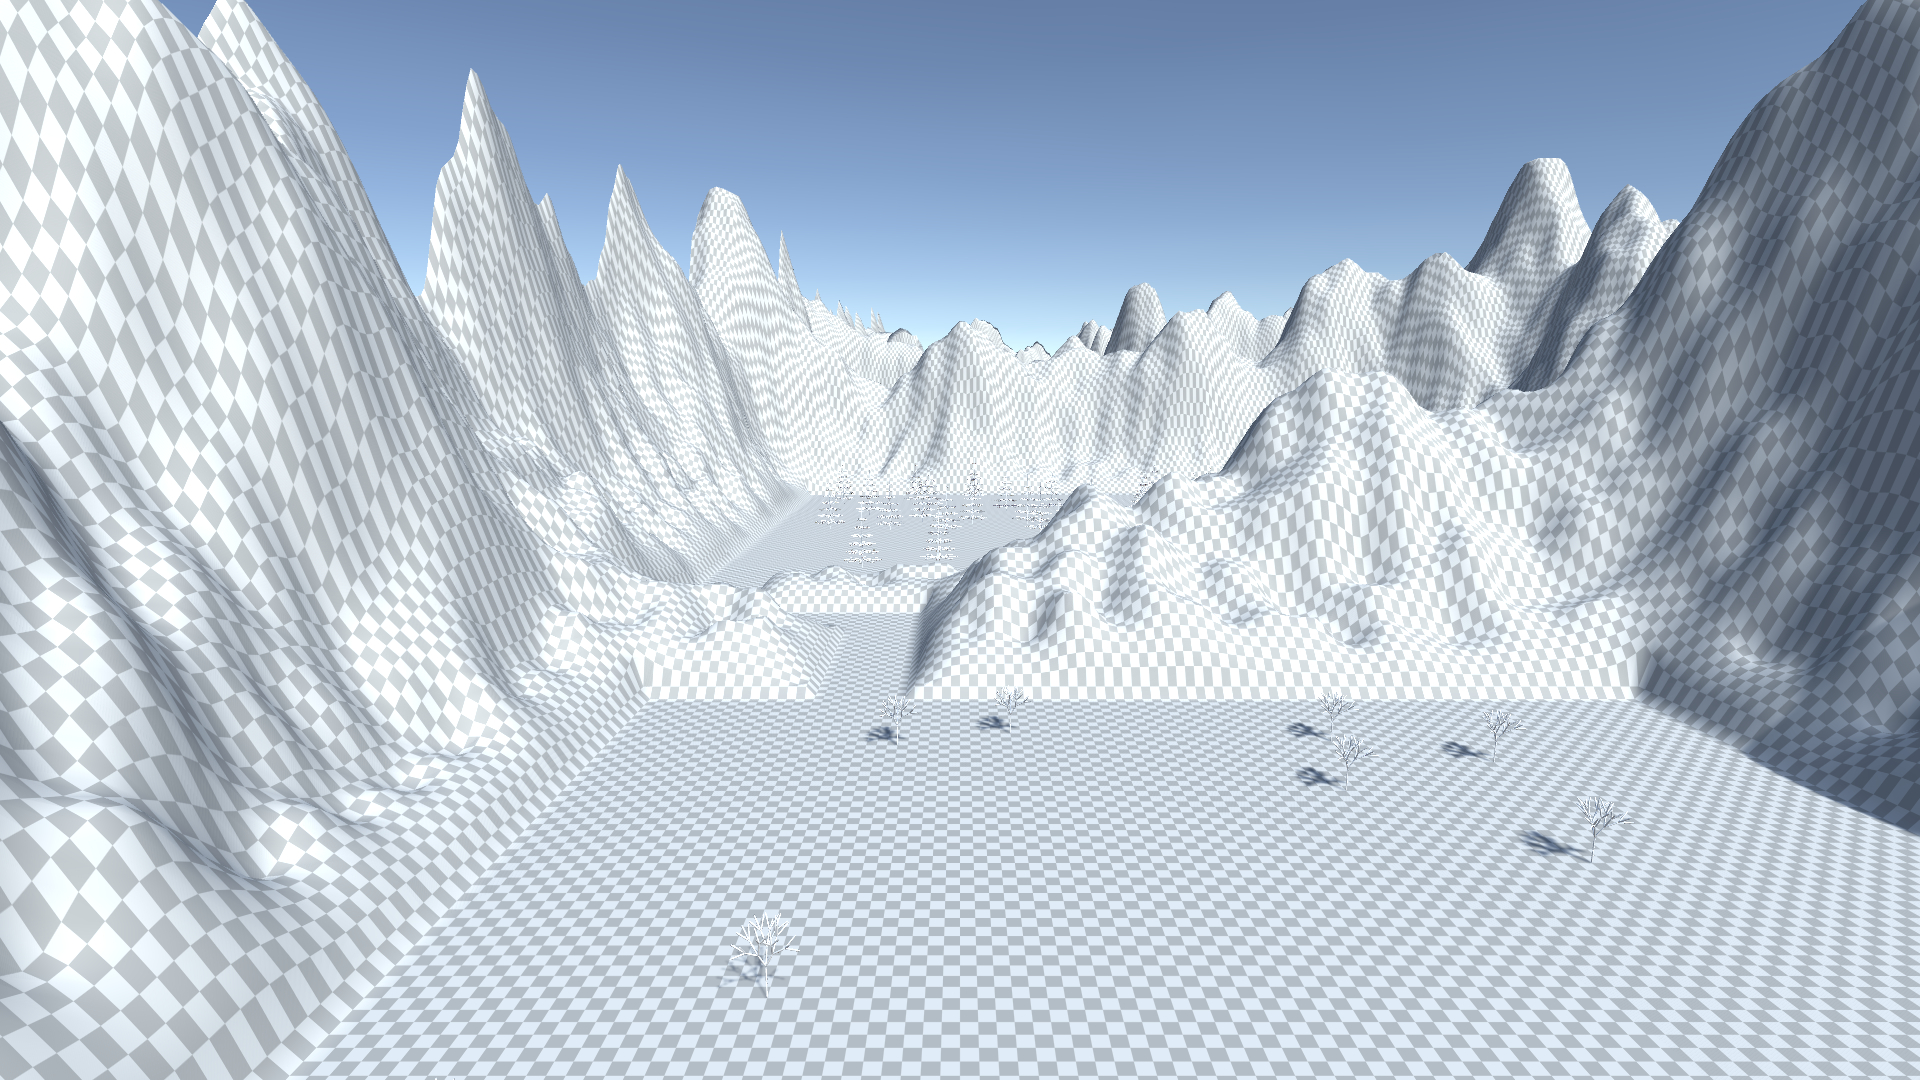
\includegraphics[width=.9\linewidth]{chapters/05_Technische_Umsetzung/03_World_Generation/Performance/fpsperfscr.png}
    \caption{Testszene für die Vegetationsmessungen}\label{fig:Vegetationscene}
\end{figure}

Im Folgenden werden die verschiedenen Optimierungen beschrieben und anhand von Messungen evaluiert.
Für jede Version wurden dabei die resultierenden Bilder pro Sekunde (FPS) und die Gesamtdauer für die Generierung erfasst.
Zusätzlich zur Gesamtdauer wurde auch die Zeit erfasst, die benötigt wird, um die GameObjects zu erzeugen und um das NavMesh zu berechnen.
Die Messungen sind in Abbildung~\ref{fig:WG::Vegetation} dargestellt.

\begin{figure}[ht]
    \centering
    \begin{tikzpicture}
        \begin{axis}[
                table/search path={chapters/05_Technische_Umsetzung/03_World_Generation/Performance},
                ybar,
                bar width=20pt,
                nodes near coords,
                % every node near coord/.append style={font=\tiny},
                % nodes near coords style={/pgf/number format/.cd,fixed,fixed zerofill,precision=0},
                % ymax=20,
                axis x line*=bottom,
                width=.9\linewidth,
                height=7.5cm,
                major grid style={dashed,black!60},
                ymajorgrids=true,
                yminorgrids=true,
                xminorgrids=false,
                symbolic x coords={1,2,3,4},
                xtick={1,2,3,4},
                xticklabels={capsules,cylinders,+combine,\textbf{+caching}},
                ymin=0,
                ytick distance=30,
                axis y line*=left,
                ylabel={FPS},
                bar shift={-\pgfplotbarwidth/2},
            ]
            \addplot[blue,semithick,fill=blue,fill opacity=0.5,text opacity=1] table [y={fps}, x={test},col sep=comma]{fps.csv};\label{FPS}
        \end{axis}
        \begin{axis}[
                table/search path={chapters/05_Technische_Umsetzung/03_World_Generation/Performance},
                ybar stacked,
                bar width=20pt,
                nodes near coords={},
                width=.9\linewidth,
                height=7.5cm,
                major grid style={dotted,black!60},
                axis on top,
                ymajorgrids=true,
                yminorgrids=true,
                xminorgrids=false,
                symbolic x coords={1,2,3,4},
                xticklabels={},
                legend style={
                        at={(0.5,1.1)},
                        anchor=north,
                        legend columns=-1,
                        fill=white,
                        align=left,
                        % font=\footnotesize,
                        minimum height=.42cm
                    },
                ymin=0,
                axis x line=none,
                axis y line*=right,
                ylabel={Laufzeit [s]},
                bar shift={\pgfplotbarwidth/2},
            ]
            \addlegendimage{/pgfplots/refstyle=FPS}\addlegendentry{FPS}
            \addplot[green,semithick,fill=green,fill opacity=0.5,text opacity=1] table [y={tgo}, x={test},col sep=comma]{fps.csv};%
            \addlegendentry{GameObject}
            \addplot[orange,semithick,fill=orange,fill opacity=0.5,text opacity=1] table [y={navmesh}, x={test},col sep=comma]{fps.csv};%
            \addlegendentry{NavMesh}
            \addplot[red,semithick,fill=red,fill opacity=0.5,text opacity=1,show sum on top] table [y={totaldiff}, x={test},col sep=comma]{fps.csv};%
            \addlegendentry{Gesamtdauer}
        \end{axis}
    \end{tikzpicture}
    \caption[Messung von Vegetationsoptimierungen]{Messungen über die resultierenden Bilder pro Sekunde (FPS) und Dauer zum Generieren des Levels mit L-System Vegetation.}\label{fig:WG::Vegetation}
\end{figure}

Die zunächst implementierte Version (capsules) folgt dem Vorgehen aus Abschnitt~\ref{sec:lsystemskel}.
Hierbei wird für jedes Segment ein neues primitives Capsule-GameObject erzeugt, welche als Kinder dem Pflanzen-Objekt angehangen werden.
Für den großen Baum resultiert dies in jeweils 121 Kind-Objekte und für den Tannenbaum in 696 Kind-Objekte.
Jedes dieser Objekte wird von Unity einzeln verarbeitet, was zu unspielbaren 8 Bildern pro Sekunde führt.
Zudem dauert es mit $\SI{19.6}{\second}$ inakzeptabel lange die Welt zu generieren.
An den Laufzeit-Anteilen ist gut erkennbar, dass die Berechnung des NavMeshes mehr als die Hälfte der Zeit in Anspruch nimmt.
Auch das Erzeugen der GameObjects hat mit ca. $\SI{7}{\second}$ einen großen Einfluss auf die Gesamtdauer.

Die erste Optimierungsidee (cylinders) war, anstatt Kapseln, Zylinder als GameObjects für die Segmente zu verwenden.
Ein \texttt{CapsuleMesh} besteht aus 832 Dreiecken, während ein \texttt{CylinderMesh} nur aus 80 Dreiecken besteht.
Dies führt zu einer erheblich verringerten Komplexität der Pflanzen, ohne dass sich das Aussehen deutlich verändert.
In der Testszene werden nun nur noch 13,1Mio. Dreiecke gerendert, anstatt der 126,5Mio. Dreiecke, wenn das \texttt{CapsuleMesh} verwendet wird.
Dies führt zwar zu einer Reduktion der Gesamtdauer auf $\SI{15.7}{\second}$, aber keiner Steigerung der Bilder pro Sekunde.
Gut zu beobachten ist hier, dass die reduzierte Komplexität der einzelnen Pflanzen auch die Berechnung des NavMeshes beschleunigt.

Damit pro Pflanze nicht mehr hunderte Kind-Objekte erstellt werden müssen, werden nun die \texttt{CylinderMeshes} der einzelnen Segmente zu einem großen Mesh kombiniert.
Das zusammengesetzte Mesh des großen Baums besteht nun aus 9680 Dreiecken und das Mesh des Tannenbaums aus 55680 Dreiecken.
Die einzelnen Meshes der Pflanzen sind also erheblich komplexer geworden, jedoch muss Unity nun nicht mehr jedes einzelne Segment als eigenes GameObject verarbeiten.
Diese Optimierung (+combine) löst die Bilder pro Sekunde Probleme, da nun 154 Bilder pro Sekunde erreicht werden.
Es ergibt sich nun jedoch ein neues Problem, da die Gesamtdauer der Generierung nun auf inakzeptable $\SI{42.1}{\second}$ steigt.
Zu erkennen ist, dass die Berechnung des NavMeshes nun ungefähr $\SI{25}{\second}$ benötigt und auch das Erzeugen der GameObjects nun länger dauert.
Die deutlich komplexeren Meshes der Pflanzen sind also ein Problem, wenn jede Pflanze ein unabhängiges GameObject ist, obwohl diese gleich aufgebaut sind.

Die letzte Optimierung (+caching) löst dieses Problem.
Es wird nun für jede Pflanze nur einmal das L-System ausgewertet und das Mesh gebildet.
Jede weitere Instanz der Pflanze wird als Klon des ursprünglichen GameObjects instanziiert.
Dies führt zu einer weiteren Steigerung auf 161 Bilder pro Sekunde und einer stark verringerten Generierungsdauer auf $\SI{4.6}{\second}$.
Durch das Klonen der Pflanzen dauert das Erzeugen der GameObjects nur noch insignifikant lang und die Berechnung des NavMeshes reduziert sich auch auf ungefähr $\SI{1}{\second}$.
Insgesamt führen die Optimierungen dazu, dass die Pflanzen zur Laufzeit prozedural generiert und platziert werden können, ohne dass sehr lange Wartezeiten entstehen.